\documentclass{article}
\usepackage[margin=0.75in]{geometry}
\usepackage{enumitem}
\usepackage{setspace}
\usepackage{amsmath}
\usepackage{amssymb}
\usepackage{physics}
\usepackage{relsize}
\usepackage{graphicx}
\usepackage{multicol}

\title{Math 174E Midterm}
\date{6/10/2021}
\author{Jiaping Zeng}

\begin{document}
\setstretch{1.35}

I certify on my honor that I have neither given nor received any help, or used any non-permitted resources, while completing this evaluation.\\
Signature: 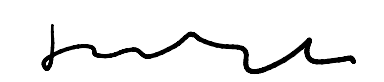
\includegraphics[width=2in]{signature.png}\\
Date: 6/10/2021
\newpage
\begin{enumerate}
      \item The spot price of gold today is \$1,890 per ounce. The current storage costs for gold are \$0.32 per ounce per year, payable quarterly in advance. Suppose the risk-free interest rate is 3\% per annum (for all maturities).\\
            Consider a forward contract on gold for delivery in 9 months.
            \begin{enumerate}
                  \item Compute today's arbitrage-free forward price of the 9-months contract.\\
                        \textbf{Answer}: The present value of the storage costs is $U_0=0.8e^{-0.03\cdot\frac{3}{12}}+0.8e^{-0.03\cdot\frac{6}{12}}+0.8e^{-0.03\cdot\frac{9}{12}}\approx 0.236$ per ounce, so we have $F_0(T)=(S_0+U_0)e^{rT}=(1890+0.236)e^{0.03\cdot\frac{9}{12}}\approx 1933.248$.
                  \item Suppose you are entering today into a long position in the 9-month forward contract on gold with the forward price computed in (a). What will be the value of the forward contract in 5 months if the gold spot price will be at \$1,700 per ounce at that time?\\
                        \textbf{Answer}: $F(T)=S_t-F_0(T)e^{-r(T-t)}=1700-1933.248e^{-0.03\cdot\frac{9-5}{12}}=-214.012$.
            \end{enumerate}
            \newpage
      \item Suppose that the price of a stock today is at \$25. For a strike price of $K=$\$24 a 3-month European call option on that stock is quoted with a price of \$2, and a 3-month European put option on the same stock is quoted at \$1.5. Assume that the risk-free rate is 10\% per annum.
            \begin{enumerate}
                  \item Does the put-call parity hold?\\
                        \textbf{Answer}: By put-call parity, the put option should be priced at $P_0=C_0+Ke^{-rT}-S_0=2+24e^{-\frac{0.3}{12}}-25\approx 0.407\neq 1.5$, so put-call parity does not hold.
                  \item Is there an arbitrage oppportunity? If yes, explain how the arbitrage strategy would look like.\\
                        \textbf{Answer}: Since put-call parity does not hold, there is an arbitrage oppportunity. We can short a put and a share while buying a call. This trade gives us $\$25+\$1.5-\$2=\$24.5$. In 3 months, either the put or the call would be in the money and we would exercise it to buy back the share for $\$24$, giving us a profit of $\$24.5-\$24=\$0.5$.
            \end{enumerate}
            \newpage
      \item Imagine you are a trader at a large investment bank and that there is a stock traded today on the stock market at a price of \$100 which will be worth tomorrow either \$120 or \$80.\\
            You have the information from a reliable source that tomorrow's price of the stock will increase to \$120 with a probability of 80\% and decrease to \$80 with a probability of 20\%. Another trader who works for a competitor is calling you and offers you to buy two put options from her on that stock for a price of \$4 per option, maturing tomorrow with a strike price of \$100.\\
            What do you do? Can you make money without any capital requirement and without any risk by trading with the other trader and the underlying stock only?\\
            Provide an explanation for your answer and assume for simplicity that the risk-free interest rate $r$ is equal to zero.\\
            \textbf{Answer}: We can replicate the put option payoff by using the following system of equations: \[\begin{cases}(V_0-100\Delta_0)+120\Delta_0=0 \\(V_0-100\Delta_0)+80\Delta_0=20\end{cases}\implies V_0=10,\Delta_0=-0.5\] So our put replication strategy is to sell $\frac{1}{2}$ share while lending away \$40. We can then short two of the replication strategies (\$20) and buy the two puts (\$8) for a risk-free gain of $\$20-\$8=\$12$.
            \newpage
      \item An \textit{asset-or-nothing stock option} is a European-style option that pays off a dollar amount equal to the stock price $S_T$ to the holder at maturity $T>0$, but only if the stock price at time $T$ is above a certain threshold $K$ (also referred to as the strike price).\\
            Suppose a stock price is currently at \$20. Assume that over each of the next two one-month periods the stock price will either go up by 5\% or go down by 5\%. The risk-free rate is 1\% p.a. with continuous compounding.\\
            Use a two-step binomial tree model to compute the arbitrage-free price of an asset-or-nothing option written on that stick with strike price \$20 and maturity 2 months.\\
            \textbf{Answer}:  $ $
            \begin{center}
                  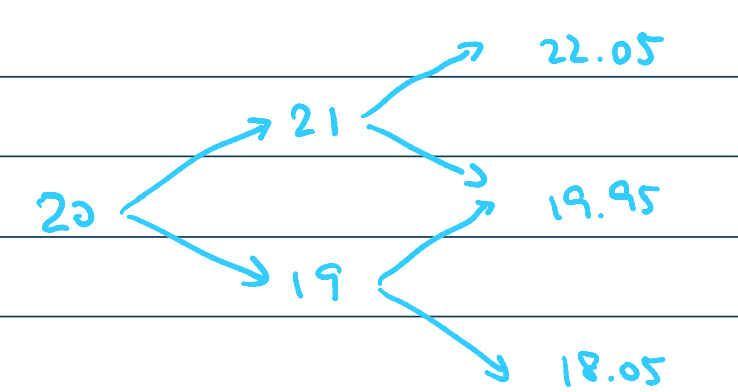
\includegraphics[width=2.5in]{4.png}
            \end{center}
            We have \[p^*=\frac{e^{\Delta t\cdot r}-d}{u-d}=\frac{e^{\frac{0.01}{12}}-0.95}{1.05-0.95}\approx 0.508\]\[1-p^*=1-0.508=0.492.\]
            At $t=2$: \[f^{uu}=22.05-20=2.05\]\[f^{ud}=f^{dd}=0.\]
            At $t=1$: \[f^u=(0.508\cdot 2.05+0.492\cdot 0)\cdot e^{\frac{0.01}{12}}\approx 1.042\]\[f^d=(0.508\cdot 0+0.492\cdot 0)\cdot e^\frac{0.01}{12}=0.\]
            Then at $t=0$ we have \[f=(0.508\cdot 1.042+0.492\cdot 0)\cdot e^{\frac{0.01}{12}}\approx 0.530.\]
            Therefore the price is \$0.530.
            \newpage
      \item A stock price is currently at \$50 and has a volatility of 30\% p.a. The risk-free interest rate is 1\% p.a. with continuous compounding.
            \begin{enumerate}
                  \item Use a three-step binomial tree model with step size 3 months to compute the arbitrage-free price of an American put option written on that stock with strike price $K=\$50$ and maturity in 9 months.\\
                        \textbf{Answer}: $ $
                        \begin{center}
                              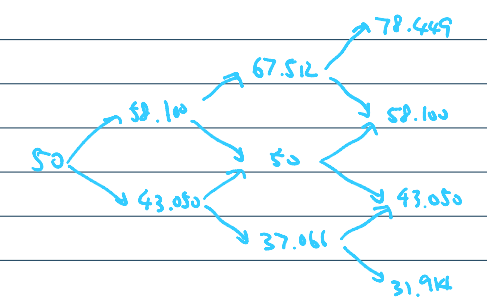
\includegraphics[width=3.5in]{5a.png}
                        \end{center}
                        We have $u=e^{\sigma\sqrt{\Delta t}}=e^{0.3\sqrt{\frac{3}{12}}}\approx 1.162$ and $d=e^{\sigma\sqrt{\Delta t}}=e^{-0.3\sqrt{\frac{3}{12}}}\approx 0.861$, so \[p^*=\frac{e^{\Delta t\cdot r}-d}{u-d}=\frac{e^{\frac{0.03}{12}}-0.861}{1.162-0.861}\approx 0.470\]\[1-p^*=1-0.470=0.530.\]
                        At $t=9$: \[g^{uuu}=g^{uud}=0\]\[g^{ddu}=50-43.050=6.950\]\[g^{ddd}=50-31.914=18.086.\]
                        At $t=6$: \[g^{uu}=0\]\[g^{ud}=(0.470\cdot 0+0.530\cdot 6.950)\cdot e^{-\frac{0.03}{12}}\approx 3.674\implies\text{take}\max(3.674,50-50)=3.674\]\[g^{dd}=(0.470\cdot 6.950+0.530\cdot 18.086)\cdot e^{-\frac{0.03}{12}}\approx 12.820\implies\text{take}\max(12.820,50-37.066)=12.934.\]
                        At $t=3$: \[g^{u}=(0.470\cdot 0+0.530\cdot 3.674)\cdot e^{-\frac{0.03}{12}}\approx 1.942\]\[g^{d}=(0.470\cdot 0+0.530\cdot 3.674)\cdot e^{-\frac{0.03}{12}}\approx 8.560\implies\text{take}\max(8.560,50-43.050)=8.560.\]
                        At $t=0$: \[g=(0.470\cdot 1.942+0.530\cdot 8.560)\cdot e^{-\frac{0.03}{12}}\approx 5.436.\]
                        Therefore the price is \$5.436.
                  \item At which nodes in the tree would it be optimal to early exercise the American put option before maturity $T$?\\
                        \textbf{Answer}: By calculations shown above, it would be optimal to early exercise at the node labeled 37.066, since $12.820<50-37.066$.
            \end{enumerate}
            \newpage
      \item Consider the Black-Scholes-Merton model where the price of a stock $S_T$ at maturity $T>0$ with initial spot price $S_0$ (today at time $t=0$) is modeled by \[S_T=S_0\cdot e^{(\mu-\frac{\sigma^2}{2})\cdot T+\sigma\cdot B_T}\] with parameters $\mu\in\mathbb{R},\sigma>0$ and normally distributed random variable $B_T\sim\mathcal{N}(0,T)$. Let $r>0$ denote the risk-free interest rate (p.a. and continuous compounded).
            \begin{enumerate}
                  \item Determine the distribution of $\log\left(\frac{S_T}{S_0}\right)$ under the ``real world'' modeling assumption and the ``risk-neutral world'' modeling assumption.\\
                        \textbf{Answer}:
                        \begin{itemize}
                              \item ``real world'': \[\log\left(\frac{S_T}{S_0}\right)=\log\left(\frac{S_0\cdot e^{(\mu-\frac{\sigma^2}{2})\cdot T+\sigma\cdot B_T}}{S_0}\right)=(\mu-\frac{\sigma^2}{2})\cdot T+\sigma\cdot B_T\]
                              \item ``risk-neutral world'': \[\log\left(\frac{S_T}{S_0}\right)=\log\left(\frac{S_0\cdot e^{(r-\frac{\sigma^2}{2})\cdot T+\sigma\cdot B_T}}{S_0}\right)=(r-\frac{\sigma^2}{2})\cdot T+\sigma\cdot B_T\]
                        \end{itemize}
                  \item Compute today's arbitrage-free price of a European-style option written on the stock which pays the holder of the option a dollar amount equal to $(S_T)^2$ at maturity $T>0$.\\
                        \textbf{Answer}: \begin{align*}
                              C_t & =\mathbb{E}[e^{-r(T-t)}(S_T-K)^+\mid S_t=s]          \\
                                  & =s\cdot\Phi(d_+(s,T-t))-Ke^{-r(T-t)}\Phi(d_-(s,T-t))
                        \end{align*}
            \end{enumerate}
\end{enumerate}

\end{document}